\Section{Allgemeines}
    \Subsection{Produktivitätskrise}
        \StandardFrame
            \begin{itemize}
                \item Systeme werden komplexer
                \item Time-To-Market soll gering bleiben
                \item Verbessern der Performance
                \begin{itemize}
                    \item Geschwindigkeit
                    \item Stromverbrauch
                \end{itemize}
                \item[]
                \item[$\rightarrow$] Produktivitätskrise
            \end{itemize}
        \end{frame}
    
    \Subsection{Grenzen der Systementwicklung}
        \StandardFrame
            \begin{itemize}
                \item Moore's law
                \item Codezeilen pro Tag pro Entwickler
                \item Physikalische Grenzen
                \item Time-To-Market
            \end{itemize}
            \vspace*{-1.3cm}
            \begin{flushright}
                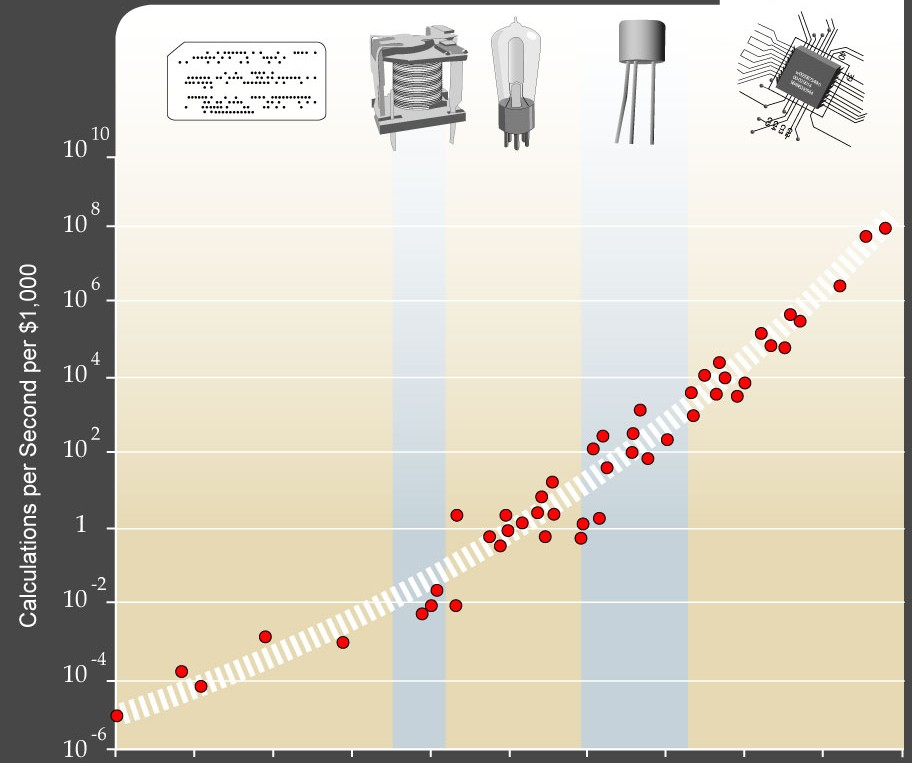
\includegraphics[scale=0.19]{pics/moores_law}
            \end{flushright}
        \end{frame}
        
    \Subsection{Kleine Verbesserungen}
        \StandardFrame
            \begin{itemize}
                \item Intelligente IDE \\
                        \quad Erzeugt Code \RA Lines of code
                \item Multi purpose IP cores \\
                        \quad \RA Lines of code
                \item[]
                \item Physikalische Grenzen \\
                        \quad Können nicht umgangen werden!
            \end{itemize}
            \vspace*{-4cm}
            \begin{flushright}
                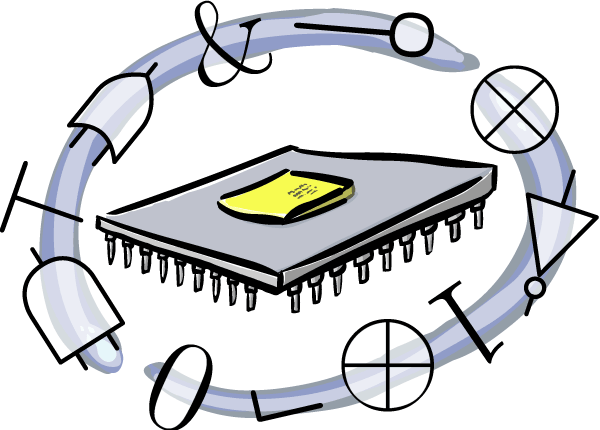
\includegraphics[scale=0.18]{pics/ipcore}
            \end{flushright}
        \end{frame}
    
    \Subsection{Abstraktion}
        \StandardFrame
            \begin{block}{Definition}
                \gray{Das Wort} Abstraktion \gray{bezeichnet meist den induktiven Denkprozess des} Weglassens von Einzelheiten und \gray{des} Überführens auf etwas \gray{Allgemeineres oder} Einfacheres.
            \end{block}
            \begin{itemize}
                \item Komplexität wird ausgeblendet
                \item Betrachtung des Wesentlichen
                \item Zurückgreifen auf bestehende Module
                \item Beeinträchtigung der Performance
            \end{itemize}
        \end{frame}
    
    \Subsection{Effizienz}
        \StandardFrame
            \begin{block}{Definition}
               	Effizienz \gray{beschreibt das} Verhältnis vom Nutzen zum Aufwand\gray{, mit welchem der Nutzen erzielt wird. Mit einem} effizienten Verhalten \gray{kann ein} größtmöglicher Nutzen beim geringst nötigen Aufwand \gray{erzielt werden.} 
            \end{block}
            \begin{itemize}
                \item Steigerung der Performance
                \item Ausnutzung spezifischer Systemeigenschaften
                \item Komplexität nimmt zu
                \item Berücksichtigung der Physik
            \end{itemize}
        \end{frame}
        
        

